% Created by tikzDevice version 0.12.6 on 2026-08-08 12:10:53
% !TEX encoding = UTF-8 Unicode
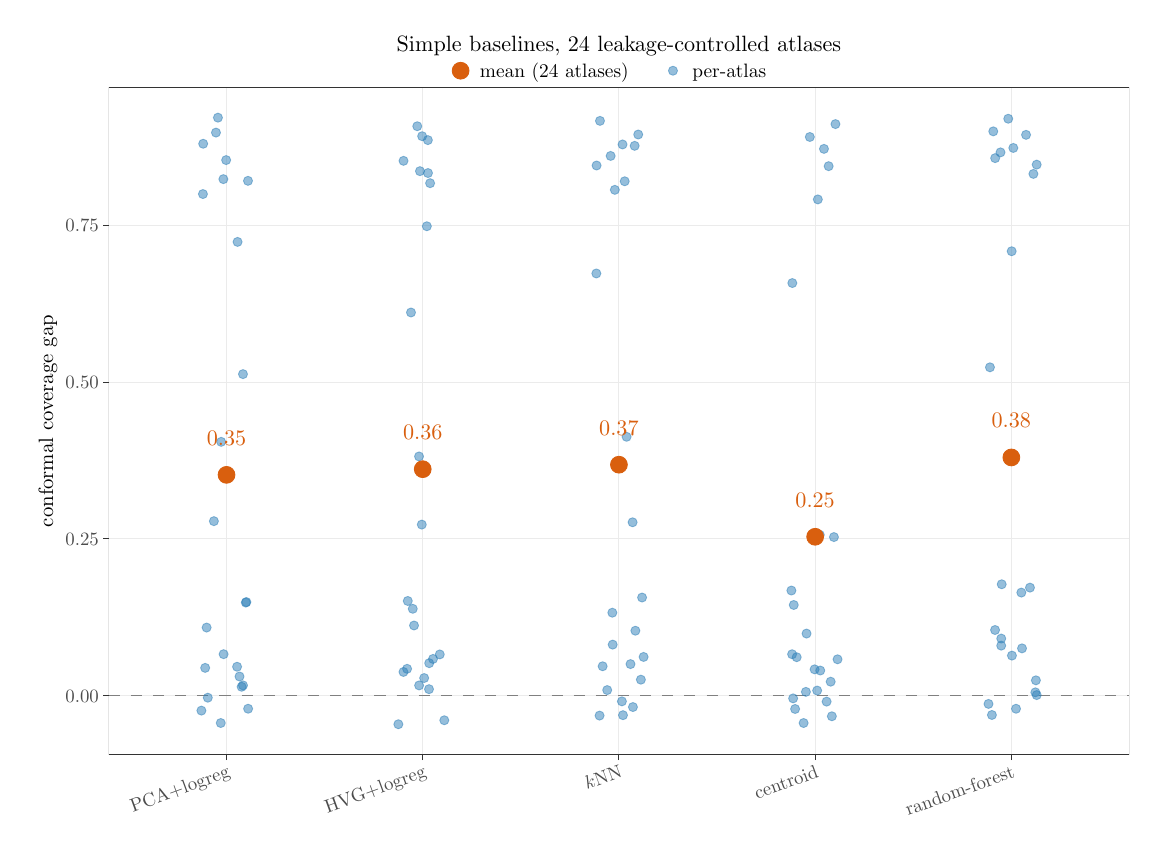
\begin{tikzpicture}[x=1pt,y=1pt]
\definecolor{fillColor}{RGB}{255,255,255}
\path[use as bounding box,fill=fillColor,fill opacity=0.00] (0,0) rectangle (403.99,289.08);
\begin{scope}
\path[clip] (  0.00,  0.00) rectangle (403.99,289.08);
\definecolor{drawColor}{RGB}{255,255,255}
\definecolor{fillColor}{RGB}{255,255,255}

\path[draw=drawColor,line width= 0.4pt,line join=round,line cap=round,fill=fillColor] (  0.00,  0.00) rectangle (403.99,289.08);
\end{scope}
\begin{scope}
\path[clip] ( 29.31, 26.41) rectangle (397.99,267.52);
\definecolor{fillColor}{RGB}{255,255,255}

\path[fill=fillColor] ( 29.31, 26.41) rectangle (397.99,267.52);
\definecolor{drawColor}{gray}{0.92}

\path[draw=drawColor,line width= 0.4pt,line join=round] ( 29.31, 47.67) --
	(397.99, 47.67);

\path[draw=drawColor,line width= 0.4pt,line join=round] ( 29.31,104.34) --
	(397.99,104.34);

\path[draw=drawColor,line width= 0.4pt,line join=round] ( 29.31,161.00) --
	(397.99,161.00);

\path[draw=drawColor,line width= 0.4pt,line join=round] ( 29.31,217.67) --
	(397.99,217.67);

\path[draw=drawColor,line width= 0.4pt,line join=round] ( 71.85, 26.41) --
	( 71.85,267.52);

\path[draw=drawColor,line width= 0.4pt,line join=round] (142.75, 26.41) --
	(142.75,267.52);

\path[draw=drawColor,line width= 0.4pt,line join=round] (213.65, 26.41) --
	(213.65,267.52);

\path[draw=drawColor,line width= 0.4pt,line join=round] (284.55, 26.41) --
	(284.55,267.52);

\path[draw=drawColor,line width= 0.4pt,line join=round] (355.45, 26.41) --
	(355.45,267.52);
\definecolor{drawColor}{gray}{0.50}

\path[draw=drawColor,line width= 0.4pt,dash pattern=on 4pt off 4pt ,line join=round] ( 29.31, 47.67) -- (397.99, 47.67);
\definecolor{drawColor}{RGB}{44,127,184}
\definecolor{fillColor}{RGB}{44,127,184}

\path[draw=drawColor,draw opacity=0.50,line width= 0.3pt,line join=round,line cap=round,fill=fillColor,fill opacity=0.50] ( 71.72,241.23) circle (  1.65);

\path[draw=drawColor,draw opacity=0.50,line width= 0.3pt,line join=round,line cap=round,fill=fillColor,fill opacity=0.50] (135.81,240.96) circle (  1.65);

\path[draw=drawColor,draw opacity=0.50,line width= 0.3pt,line join=round,line cap=round,fill=fillColor,fill opacity=0.50] (210.65,242.73) circle (  1.65);

\path[draw=drawColor,draw opacity=0.50,line width= 0.3pt,line join=round,line cap=round,fill=fillColor,fill opacity=0.50] (285.52,227.02) circle (  1.65);

\path[draw=drawColor,draw opacity=0.50,line width= 0.3pt,line join=round,line cap=round,fill=fillColor,fill opacity=0.50] (351.53,244.02) circle (  1.65);

\path[draw=drawColor,draw opacity=0.50,line width= 0.3pt,line join=round,line cap=round,fill=fillColor,fill opacity=0.50] ( 79.61,233.73) circle (  1.65);

\path[draw=drawColor,draw opacity=0.50,line width= 0.3pt,line join=round,line cap=round,fill=fillColor,fill opacity=0.50] (141.75,237.23) circle (  1.65);

\path[draw=drawColor,draw opacity=0.50,line width= 0.3pt,line join=round,line cap=round,fill=fillColor,fill opacity=0.50] (205.57,239.27) circle (  1.65);

\path[draw=drawColor,draw opacity=0.50,line width= 0.3pt,line join=round,line cap=round,fill=fillColor,fill opacity=0.50] (289.43,239.03) circle (  1.65);

\path[draw=drawColor,draw opacity=0.50,line width= 0.3pt,line join=round,line cap=round,fill=fillColor,fill opacity=0.50] (363.42,236.24) circle (  1.65);

\path[draw=drawColor,draw opacity=0.50,line width= 0.3pt,line join=round,line cap=round,fill=fillColor,fill opacity=0.50] ( 77.80,163.89) circle (  1.65);

\path[draw=drawColor,draw opacity=0.50,line width= 0.3pt,line join=round,line cap=round,fill=fillColor,fill opacity=0.50] (138.51,186.16) circle (  1.65);

\path[draw=drawColor,draw opacity=0.50,line width= 0.3pt,line join=round,line cap=round,fill=fillColor,fill opacity=0.50] (205.49,200.26) circle (  1.65);

\path[draw=drawColor,draw opacity=0.50,line width= 0.3pt,line join=round,line cap=round,fill=fillColor,fill opacity=0.50] (276.22, 62.67) circle (  1.65);

\path[draw=drawColor,draw opacity=0.50,line width= 0.3pt,line join=round,line cap=round,fill=fillColor,fill opacity=0.50] (355.56,208.29) circle (  1.65);

\path[draw=drawColor,draw opacity=0.50,line width= 0.3pt,line join=round,line cap=round,fill=fillColor,fill opacity=0.50] ( 62.78, 42.30) circle (  1.65);

\path[draw=drawColor,draw opacity=0.50,line width= 0.3pt,line join=round,line cap=round,fill=fillColor,fill opacity=0.50] (150.55, 38.81) circle (  1.65);

\path[draw=drawColor,draw opacity=0.50,line width= 0.3pt,line join=round,line cap=round,fill=fillColor,fill opacity=0.50] (218.71, 43.59) circle (  1.65);

\path[draw=drawColor,draw opacity=0.50,line width= 0.3pt,line join=round,line cap=round,fill=fillColor,fill opacity=0.50] (280.38, 37.82) circle (  1.65);

\path[draw=drawColor,draw opacity=0.50,line width= 0.3pt,line join=round,line cap=round,fill=fillColor,fill opacity=0.50] (357.14, 42.97) circle (  1.65);

\path[draw=drawColor,draw opacity=0.50,line width= 0.3pt,line join=round,line cap=round,fill=fillColor,fill opacity=0.50] ( 77.31, 50.91) circle (  1.65);

\path[draw=drawColor,draw opacity=0.50,line width= 0.3pt,line join=round,line cap=round,fill=fillColor,fill opacity=0.50] (135.79, 56.27) circle (  1.65);

\path[draw=drawColor,draw opacity=0.50,line width= 0.3pt,line join=round,line cap=round,fill=fillColor,fill opacity=0.50] (222.56, 61.69) circle (  1.65);

\path[draw=drawColor,draw opacity=0.50,line width= 0.3pt,line join=round,line cap=round,fill=fillColor,fill opacity=0.50] (286.40, 56.78) circle (  1.65);

\path[draw=drawColor,draw opacity=0.50,line width= 0.3pt,line join=round,line cap=round,fill=fillColor,fill opacity=0.50] (349.56, 71.43) circle (  1.65);

\path[draw=drawColor,draw opacity=0.50,line width= 0.3pt,line join=round,line cap=round,fill=fillColor,fill opacity=0.50] ( 68.04,251.17) circle (  1.65);

\path[draw=drawColor,draw opacity=0.50,line width= 0.3pt,line join=round,line cap=round,fill=fillColor,fill opacity=0.50] (142.54,249.86) circle (  1.65);

\path[draw=drawColor,draw opacity=0.50,line width= 0.3pt,line join=round,line cap=round,fill=fillColor,fill opacity=0.50] (220.62,250.47) circle (  1.65);

\path[draw=drawColor,draw opacity=0.50,line width= 0.3pt,line join=round,line cap=round,fill=fillColor,fill opacity=0.50] (287.74,245.28) circle (  1.65);

\path[draw=drawColor,draw opacity=0.50,line width= 0.3pt,line join=round,line cap=round,fill=fillColor,fill opacity=0.50] (348.92,251.61) circle (  1.65);

\path[draw=drawColor,draw opacity=0.50,line width= 0.3pt,line join=round,line cap=round,fill=fillColor,fill opacity=0.50] ( 69.92,139.42) circle (  1.65);

\path[draw=drawColor,draw opacity=0.50,line width= 0.3pt,line join=round,line cap=round,fill=fillColor,fill opacity=0.50] (141.42,134.14) circle (  1.65);

\path[draw=drawColor,draw opacity=0.50,line width= 0.3pt,line join=round,line cap=round,fill=fillColor,fill opacity=0.50] (216.41,141.24) circle (  1.65);

\path[draw=drawColor,draw opacity=0.50,line width= 0.3pt,line join=round,line cap=round,fill=fillColor,fill opacity=0.50] (291.34,105.01) circle (  1.65);

\path[draw=drawColor,draw opacity=0.50,line width= 0.3pt,line join=round,line cap=round,fill=fillColor,fill opacity=0.50] (347.72,166.35) circle (  1.65);

\path[draw=drawColor,draw opacity=0.50,line width= 0.3pt,line join=round,line cap=round,fill=fillColor,fill opacity=0.50] ( 63.42,247.13) circle (  1.65);

\path[draw=drawColor,draw opacity=0.50,line width= 0.3pt,line join=round,line cap=round,fill=fillColor,fill opacity=0.50] (144.61,248.45) circle (  1.65);

\path[draw=drawColor,draw opacity=0.50,line width= 0.3pt,line join=round,line cap=round,fill=fillColor,fill opacity=0.50] (219.33,246.38) circle (  1.65);

\path[draw=drawColor,draw opacity=0.50,line width= 0.3pt,line join=round,line cap=round,fill=fillColor,fill opacity=0.50] (282.63,249.58) circle (  1.65);

\path[draw=drawColor,draw opacity=0.50,line width= 0.3pt,line join=round,line cap=round,fill=fillColor,fill opacity=0.50] (356.16,245.62) circle (  1.65);

\path[draw=drawColor,draw opacity=0.50,line width= 0.3pt,line join=round,line cap=round,fill=fillColor,fill opacity=0.50] ( 77.81, 51.42) circle (  1.65);

\path[draw=drawColor,draw opacity=0.50,line width= 0.3pt,line join=round,line cap=round,fill=fillColor,fill opacity=0.50] (142.41,109.52) circle (  1.65);

\path[draw=drawColor,draw opacity=0.50,line width= 0.3pt,line join=round,line cap=round,fill=fillColor,fill opacity=0.50] (218.58,110.35) circle (  1.65);

\path[draw=drawColor,draw opacity=0.50,line width= 0.3pt,line join=round,line cap=round,fill=fillColor,fill opacity=0.50] (275.97, 85.69) circle (  1.65);

\path[draw=drawColor,draw opacity=0.50,line width= 0.3pt,line join=round,line cap=round,fill=fillColor,fill opacity=0.50] (362.18, 86.74) circle (  1.65);

\path[draw=drawColor,draw opacity=0.50,line width= 0.3pt,line join=round,line cap=round,fill=fillColor,fill opacity=0.50] ( 78.82, 81.34) circle (  1.65);

\path[draw=drawColor,draw opacity=0.50,line width= 0.3pt,line join=round,line cap=round,fill=fillColor,fill opacity=0.50] (137.35, 81.92) circle (  1.65);

\path[draw=drawColor,draw opacity=0.50,line width= 0.3pt,line join=round,line cap=round,fill=fillColor,fill opacity=0.50] (211.27, 77.68) circle (  1.65);

\path[draw=drawColor,draw opacity=0.50,line width= 0.3pt,line join=round,line cap=round,fill=fillColor,fill opacity=0.50] (276.82, 80.47) circle (  1.65);

\path[draw=drawColor,draw opacity=0.50,line width= 0.3pt,line join=round,line cap=round,fill=fillColor,fill opacity=0.50] (351.96, 87.95) circle (  1.65);

\path[draw=drawColor,draw opacity=0.50,line width= 0.3pt,line join=round,line cap=round,fill=fillColor,fill opacity=0.50] ( 69.77, 37.82) circle (  1.65);

\path[draw=drawColor,draw opacity=0.50,line width= 0.3pt,line join=round,line cap=round,fill=fillColor,fill opacity=0.50] (133.95, 37.37) circle (  1.65);

\path[draw=drawColor,draw opacity=0.50,line width= 0.3pt,line join=round,line cap=round,fill=fillColor,fill opacity=0.50] (206.65, 40.50) circle (  1.65);

\path[draw=drawColor,draw opacity=0.50,line width= 0.3pt,line join=round,line cap=round,fill=fillColor,fill opacity=0.50] (276.59, 46.72) circle (  1.65);

\path[draw=drawColor,draw opacity=0.50,line width= 0.3pt,line join=round,line cap=round,fill=fillColor,fill opacity=0.50] (348.43, 40.72) circle (  1.65);

\path[draw=drawColor,draw opacity=0.50,line width= 0.3pt,line join=round,line cap=round,fill=fillColor,fill opacity=0.50] ( 79.03, 81.53) circle (  1.65);

\path[draw=drawColor,draw opacity=0.50,line width= 0.3pt,line join=round,line cap=round,fill=fillColor,fill opacity=0.50] (139.15, 79.09) circle (  1.65);

\path[draw=drawColor,draw opacity=0.50,line width= 0.3pt,line join=round,line cap=round,fill=fillColor,fill opacity=0.50] (217.83, 59.11) circle (  1.65);

\path[draw=drawColor,draw opacity=0.50,line width= 0.3pt,line join=round,line cap=round,fill=fillColor,fill opacity=0.50] (284.35, 57.21) circle (  1.65);

\path[draw=drawColor,draw opacity=0.50,line width= 0.3pt,line join=round,line cap=round,fill=fillColor,fill opacity=0.50] (351.78, 65.78) circle (  1.65);

\path[draw=drawColor,draw opacity=0.50,line width= 0.3pt,line join=round,line cap=round,fill=fillColor,fill opacity=0.50] ( 68.75,256.56) circle (  1.65);

\path[draw=drawColor,draw opacity=0.50,line width= 0.3pt,line join=round,line cap=round,fill=fillColor,fill opacity=0.50] (140.78,253.46) circle (  1.65);

\path[draw=drawColor,draw opacity=0.50,line width= 0.3pt,line join=round,line cap=round,fill=fillColor,fill opacity=0.50] (206.80,255.40) circle (  1.65);

\path[draw=drawColor,draw opacity=0.50,line width= 0.3pt,line join=round,line cap=round,fill=fillColor,fill opacity=0.50] (291.89,254.24) circle (  1.65);

\path[draw=drawColor,draw opacity=0.50,line width= 0.3pt,line join=round,line cap=round,fill=fillColor,fill opacity=0.50] (354.33,256.17) circle (  1.65);

\path[draw=drawColor,draw opacity=0.50,line width= 0.3pt,line join=round,line cap=round,fill=fillColor,fill opacity=0.50] ( 67.29,110.76) circle (  1.65);

\path[draw=drawColor,draw opacity=0.50,line width= 0.3pt,line join=round,line cap=round,fill=fillColor,fill opacity=0.50] (137.10, 57.40) circle (  1.65);

\path[draw=drawColor,draw opacity=0.50,line width= 0.3pt,line join=round,line cap=round,fill=fillColor,fill opacity=0.50] (211.39, 66.15) circle (  1.65);

\path[draw=drawColor,draw opacity=0.50,line width= 0.3pt,line join=round,line cap=round,fill=fillColor,fill opacity=0.50] (286.23,105.82) circle (  1.65);

\path[draw=drawColor,draw opacity=0.50,line width= 0.3pt,line join=round,line cap=round,fill=fillColor,fill opacity=0.50] (359.06, 84.95) circle (  1.65);

\path[draw=drawColor,draw opacity=0.50,line width= 0.3pt,line join=round,line cap=round,fill=fillColor,fill opacity=0.50] ( 65.09, 46.97) circle (  1.65);

\path[draw=drawColor,draw opacity=0.50,line width= 0.3pt,line join=round,line cap=round,fill=fillColor,fill opacity=0.50] (141.45, 51.40) circle (  1.65);

\path[draw=drawColor,draw opacity=0.50,line width= 0.3pt,line join=round,line cap=round,fill=fillColor,fill opacity=0.50] (214.72, 45.64) circle (  1.65);

\path[draw=drawColor,draw opacity=0.50,line width= 0.3pt,line join=round,line cap=round,fill=fillColor,fill opacity=0.50] (288.69, 45.55) circle (  1.65);

\path[draw=drawColor,draw opacity=0.50,line width= 0.3pt,line join=round,line cap=round,fill=fillColor,fill opacity=0.50] (364.13, 48.90) circle (  1.65);

\path[draw=drawColor,draw opacity=0.50,line width= 0.3pt,line join=round,line cap=round,fill=fillColor,fill opacity=0.50] ( 79.66, 42.98) circle (  1.65);

\path[draw=drawColor,draw opacity=0.50,line width= 0.3pt,line join=round,line cap=round,fill=fillColor,fill opacity=0.50] (145.02, 50.05) circle (  1.65);

\path[draw=drawColor,draw opacity=0.50,line width= 0.3pt,line join=round,line cap=round,fill=fillColor,fill opacity=0.50] (209.41, 49.72) circle (  1.65);

\path[draw=drawColor,draw opacity=0.50,line width= 0.3pt,line join=round,line cap=round,fill=fillColor,fill opacity=0.50] (281.21, 49.07) circle (  1.65);

\path[draw=drawColor,draw opacity=0.50,line width= 0.3pt,line join=round,line cap=round,fill=fillColor,fill opacity=0.50] (364.61, 47.91) circle (  1.65);

\path[draw=drawColor,draw opacity=0.50,line width= 0.3pt,line join=round,line cap=round,fill=fillColor,fill opacity=0.50] ( 63.33,228.96) circle (  1.65);

\path[draw=drawColor,draw opacity=0.50,line width= 0.3pt,line join=round,line cap=round,fill=fillColor,fill opacity=0.50] (145.42,232.88) circle (  1.65);

\path[draw=drawColor,draw opacity=0.50,line width= 0.3pt,line join=round,line cap=round,fill=fillColor,fill opacity=0.50] (212.17,230.48) circle (  1.65);

\path[draw=drawColor,draw opacity=0.50,line width= 0.3pt,line join=round,line cap=round,fill=fillColor,fill opacity=0.50] (281.44, 70.14) circle (  1.65);

\path[draw=drawColor,draw opacity=0.50,line width= 0.3pt,line join=round,line cap=round,fill=fillColor,fill opacity=0.50] (364.60,239.59) circle (  1.65);

\path[draw=drawColor,draw opacity=0.50,line width= 0.3pt,line join=round,line cap=round,fill=fillColor,fill opacity=0.50] ( 64.66, 72.31) circle (  1.65);

\path[draw=drawColor,draw opacity=0.50,line width= 0.3pt,line join=round,line cap=round,fill=fillColor,fill opacity=0.50] (139.61, 73.06) circle (  1.65);

\path[draw=drawColor,draw opacity=0.50,line width= 0.3pt,line join=round,line cap=round,fill=fillColor,fill opacity=0.50] (222.01, 83.16) circle (  1.65);

\path[draw=drawColor,draw opacity=0.50,line width= 0.3pt,line join=round,line cap=round,fill=fillColor,fill opacity=0.50] (277.31, 42.89) circle (  1.65);

\path[draw=drawColor,draw opacity=0.50,line width= 0.3pt,line join=round,line cap=round,fill=fillColor,fill opacity=0.50] (359.30, 64.79) circle (  1.65);

\path[draw=drawColor,draw opacity=0.50,line width= 0.3pt,line join=round,line cap=round,fill=fillColor,fill opacity=0.50] ( 64.14, 57.74) circle (  1.65);

\path[draw=drawColor,draw opacity=0.50,line width= 0.3pt,line join=round,line cap=round,fill=fillColor,fill opacity=0.50] (145.09, 59.44) circle (  1.65);

\path[draw=drawColor,draw opacity=0.50,line width= 0.3pt,line join=round,line cap=round,fill=fillColor,fill opacity=0.50] (207.76, 58.32) circle (  1.65);

\path[draw=drawColor,draw opacity=0.50,line width= 0.3pt,line join=round,line cap=round,fill=fillColor,fill opacity=0.50] (277.88, 61.60) circle (  1.65);

\path[draw=drawColor,draw opacity=0.50,line width= 0.3pt,line join=round,line cap=round,fill=fillColor,fill opacity=0.50] (355.66, 62.18) circle (  1.65);

\path[draw=drawColor,draw opacity=0.50,line width= 0.3pt,line join=round,line cap=round,fill=fillColor,fill opacity=0.50] ( 75.84,211.66) circle (  1.65);

\path[draw=drawColor,draw opacity=0.50,line width= 0.3pt,line join=round,line cap=round,fill=fillColor,fill opacity=0.50] (144.24,217.32) circle (  1.65);

\path[draw=drawColor,draw opacity=0.50,line width= 0.3pt,line join=round,line cap=round,fill=fillColor,fill opacity=0.50] (215.73,233.57) circle (  1.65);

\path[draw=drawColor,draw opacity=0.50,line width= 0.3pt,line join=round,line cap=round,fill=fillColor,fill opacity=0.50] (276.31,196.80) circle (  1.65);

\path[draw=drawColor,draw opacity=0.50,line width= 0.3pt,line join=round,line cap=round,fill=fillColor,fill opacity=0.50] (349.60,241.94) circle (  1.65);

\path[draw=drawColor,draw opacity=0.50,line width= 0.3pt,line join=round,line cap=round,fill=fillColor,fill opacity=0.50] ( 70.80, 62.69) circle (  1.65);

\path[draw=drawColor,draw opacity=0.50,line width= 0.3pt,line join=round,line cap=round,fill=fillColor,fill opacity=0.50] (146.47, 60.97) circle (  1.65);

\path[draw=drawColor,draw opacity=0.50,line width= 0.3pt,line join=round,line cap=round,fill=fillColor,fill opacity=0.50] (221.58, 53.48) circle (  1.65);

\path[draw=drawColor,draw opacity=0.50,line width= 0.3pt,line join=round,line cap=round,fill=fillColor,fill opacity=0.50] (290.16, 52.75) circle (  1.65);

\path[draw=drawColor,draw opacity=0.50,line width= 0.3pt,line join=round,line cap=round,fill=fillColor,fill opacity=0.50] (364.32, 53.24) circle (  1.65);

\path[draw=drawColor,draw opacity=0.50,line width= 0.3pt,line join=round,line cap=round,fill=fillColor,fill opacity=0.50] ( 75.67, 58.15) circle (  1.65);

\path[draw=drawColor,draw opacity=0.50,line width= 0.3pt,line join=round,line cap=round,fill=fillColor,fill opacity=0.50] (143.27, 54.07) circle (  1.65);

\path[draw=drawColor,draw opacity=0.50,line width= 0.3pt,line join=round,line cap=round,fill=fillColor,fill opacity=0.50] (215.11, 40.65) circle (  1.65);

\path[draw=drawColor,draw opacity=0.50,line width= 0.3pt,line join=round,line cap=round,fill=fillColor,fill opacity=0.50] (290.59, 40.25) circle (  1.65);

\path[draw=drawColor,draw opacity=0.50,line width= 0.3pt,line join=round,line cap=round,fill=fillColor,fill opacity=0.50] (347.19, 44.72) circle (  1.65);

\path[draw=drawColor,draw opacity=0.50,line width= 0.3pt,line join=round,line cap=round,fill=fillColor,fill opacity=0.50] ( 76.55, 54.63) circle (  1.65);

\path[draw=drawColor,draw opacity=0.50,line width= 0.3pt,line join=round,line cap=round,fill=fillColor,fill opacity=0.50] (148.91, 62.60) circle (  1.65);

\path[draw=drawColor,draw opacity=0.50,line width= 0.3pt,line join=round,line cap=round,fill=fillColor,fill opacity=0.50] (219.60, 71.17) circle (  1.65);

\path[draw=drawColor,draw opacity=0.50,line width= 0.3pt,line join=round,line cap=round,fill=fillColor,fill opacity=0.50] (292.64, 60.84) circle (  1.65);

\path[draw=drawColor,draw opacity=0.50,line width= 0.3pt,line join=round,line cap=round,fill=fillColor,fill opacity=0.50] (351.80, 68.34) circle (  1.65);

\path[draw=drawColor,draw opacity=0.50,line width= 0.3pt,line join=round,line cap=round,fill=fillColor,fill opacity=0.50] ( 70.72,234.35) circle (  1.65);

\path[draw=drawColor,draw opacity=0.50,line width= 0.3pt,line join=round,line cap=round,fill=fillColor,fill opacity=0.50] (144.65,236.55) circle (  1.65);

\path[draw=drawColor,draw opacity=0.50,line width= 0.3pt,line join=round,line cap=round,fill=fillColor,fill opacity=0.50] (214.95,246.88) circle (  1.65);

\path[draw=drawColor,draw opacity=0.50,line width= 0.3pt,line join=round,line cap=round,fill=fillColor,fill opacity=0.50] (285.28, 49.55) circle (  1.65);

\path[draw=drawColor,draw opacity=0.50,line width= 0.3pt,line join=round,line cap=round,fill=fillColor,fill opacity=0.50] (360.76,250.35) circle (  1.65);
\definecolor{drawColor}{RGB}{217,95,14}
\definecolor{fillColor}{RGB}{217,95,14}

\path[draw=drawColor,line width= 0.3pt,line join=round,line cap=round,fill=fillColor] ( 71.85,127.49) circle (  3.04);

\path[draw=drawColor,line width= 0.3pt,line join=round,line cap=round,fill=fillColor] (142.75,129.54) circle (  3.04);

\path[draw=drawColor,line width= 0.3pt,line join=round,line cap=round,fill=fillColor] (213.65,131.16) circle (  3.04);

\path[draw=drawColor,line width= 0.3pt,line join=round,line cap=round,fill=fillColor] (284.55,105.12) circle (  3.04);

\path[draw=drawColor,line width= 0.3pt,line join=round,line cap=round,fill=fillColor] (355.45,133.78) circle (  3.04);

\node[text=drawColor,anchor=base,inner sep=0pt, outer sep=0pt, scale=  0.80] at ( 71.85,138.19) {0.35};

\node[text=drawColor,anchor=base,inner sep=0pt, outer sep=0pt, scale=  0.80] at (142.75,140.24) {0.36};

\node[text=drawColor,anchor=base,inner sep=0pt, outer sep=0pt, scale=  0.80] at (213.65,141.86) {0.37};

\node[text=drawColor,anchor=base,inner sep=0pt, outer sep=0pt, scale=  0.80] at (284.55,115.82) {0.25};

\node[text=drawColor,anchor=base,inner sep=0pt, outer sep=0pt, scale=  0.80] at (355.45,144.48) {0.38};
\definecolor{drawColor}{gray}{0.20}

\path[draw=drawColor,line width= 0.4pt,line join=round,line cap=round] ( 29.31, 26.41) rectangle (397.99,267.52);
\end{scope}
\begin{scope}
\path[clip] (  0.00,  0.00) rectangle (403.99,289.08);
\definecolor{drawColor}{gray}{0.30}

\node[text=drawColor,anchor=base east,inner sep=0pt, outer sep=0pt, scale=  0.68] at ( 25.71, 45.33) {0.00};

\node[text=drawColor,anchor=base east,inner sep=0pt, outer sep=0pt, scale=  0.68] at ( 25.71,101.99) {0.25};

\node[text=drawColor,anchor=base east,inner sep=0pt, outer sep=0pt, scale=  0.68] at ( 25.71,158.66) {0.50};

\node[text=drawColor,anchor=base east,inner sep=0pt, outer sep=0pt, scale=  0.68] at ( 25.71,215.33) {0.75};
\end{scope}
\begin{scope}
\path[clip] (  0.00,  0.00) rectangle (403.99,289.08);
\definecolor{drawColor}{gray}{0.20}

\path[draw=drawColor,line width= 0.4pt,line join=round] ( 27.31, 47.67) --
	( 29.31, 47.67);

\path[draw=drawColor,line width= 0.4pt,line join=round] ( 27.31,104.34) --
	( 29.31,104.34);

\path[draw=drawColor,line width= 0.4pt,line join=round] ( 27.31,161.00) --
	( 29.31,161.00);

\path[draw=drawColor,line width= 0.4pt,line join=round] ( 27.31,217.67) --
	( 29.31,217.67);
\end{scope}
\begin{scope}
\path[clip] (  0.00,  0.00) rectangle (403.99,289.08);
\definecolor{drawColor}{gray}{0.20}

\path[draw=drawColor,line width= 0.4pt,line join=round] ( 71.85, 24.41) --
	( 71.85, 26.41);

\path[draw=drawColor,line width= 0.4pt,line join=round] (142.75, 24.41) --
	(142.75, 26.41);

\path[draw=drawColor,line width= 0.4pt,line join=round] (213.65, 24.41) --
	(213.65, 26.41);

\path[draw=drawColor,line width= 0.4pt,line join=round] (284.55, 24.41) --
	(284.55, 26.41);

\path[draw=drawColor,line width= 0.4pt,line join=round] (355.45, 24.41) --
	(355.45, 26.41);
\end{scope}
\begin{scope}
\path[clip] (  0.00,  0.00) rectangle (403.99,289.08);
\definecolor{drawColor}{gray}{0.30}

\node[text=drawColor,rotate= 20.00,anchor=base east,inner sep=0pt, outer sep=0pt, scale=  0.68] at ( 73.45, 18.41) {PCA+logreg};

\node[text=drawColor,rotate= 20.00,anchor=base east,inner sep=0pt, outer sep=0pt, scale=  0.68] at (144.35, 18.41) {HVG+logreg};

\node[text=drawColor,rotate= 20.00,anchor=base east,inner sep=0pt, outer sep=0pt, scale=  0.68] at (215.25, 18.41) {$k$NN};

\node[text=drawColor,rotate= 20.00,anchor=base east,inner sep=0pt, outer sep=0pt, scale=  0.68] at (286.15, 18.41) {centroid};

\node[text=drawColor,rotate= 20.00,anchor=base east,inner sep=0pt, outer sep=0pt, scale=  0.68] at (357.05, 18.41) {random-forest};
\end{scope}
\begin{scope}
\path[clip] (  0.00,  0.00) rectangle (403.99,289.08);
\definecolor{drawColor}{RGB}{0,0,0}

\node[text=drawColor,rotate= 90.00,anchor=base,inner sep=0pt, outer sep=0pt, scale=  0.75] at (  9.17,146.96) {conformal coverage gap};
\end{scope}
\begin{scope}
\path[clip] (  0.00,  0.00) rectangle (403.99,289.08);
\definecolor{fillColor}{RGB}{255,255,255}

\path[fill=fillColor] (151.44,269.52) rectangle (275.86,277.52);
\end{scope}
\begin{scope}
\path[clip] (  0.00,  0.00) rectangle (403.99,289.08);
\definecolor{fillColor}{RGB}{255,255,255}

\path[fill=fillColor] (152.44,269.52) rectangle (160.44,277.52);
\definecolor{drawColor}{RGB}{217,95,14}
\definecolor{fillColor}{RGB}{217,95,14}

\path[draw=drawColor,line width= 0.3pt,line join=round,line cap=round,fill=fillColor] (156.44,273.52) circle (  3.04);
\end{scope}
\begin{scope}
\path[clip] (  0.00,  0.00) rectangle (403.99,289.08);
\definecolor{fillColor}{RGB}{255,255,255}

\path[fill=fillColor] (229.17,269.52) rectangle (237.17,277.52);
\definecolor{drawColor}{RGB}{44,127,184}
\definecolor{fillColor}{RGB}{44,127,184}

\path[draw=drawColor,draw opacity=0.50,line width= 0.3pt,line join=round,line cap=round,fill=fillColor,fill opacity=0.50] (233.17,273.52) circle (  1.65);
\end{scope}
\begin{scope}
\path[clip] (  0.00,  0.00) rectangle (403.99,289.08);
\definecolor{drawColor}{RGB}{0,0,0}

\node[text=drawColor,anchor=base west,inner sep=0pt, outer sep=0pt, scale=  0.70] at (163.44,271.10) {mean (24 atlases)};
\end{scope}
\begin{scope}
\path[clip] (  0.00,  0.00) rectangle (403.99,289.08);
\definecolor{drawColor}{RGB}{0,0,0}

\node[text=drawColor,anchor=base west,inner sep=0pt, outer sep=0pt, scale=  0.70] at (240.17,271.10) {per-atlas};
\end{scope}
\begin{scope}
\path[clip] (  0.00,  0.00) rectangle (403.99,289.08);
\definecolor{drawColor}{RGB}{0,0,0}

\node[text=drawColor,anchor=base,inner sep=0pt, outer sep=0pt, scale=  0.80] at (213.65,280.57) {Simple baselines, 24 leakage-controlled atlases};
\end{scope}
\end{tikzpicture}
